\documentclass{article}
\usepackage{graphicx}
\usepackage{siunitx} 
\usepackage{natbib}
\usepackage{mathtools}
\usepackage{amssymb}
\usepackage{amsthm}
\usepackage{stackengine}
\usepackage{graphicx,ifthen}
\usepackage{amsmath}
\usepackage{braket}
\usepackage{float}
\usepackage{cancel}
\usepackage{anyfontsize}
\usepackage{scalefnt}
\usepackage{tipa}
\usepackage{multirow}
\usepackage{array}
\usepackage{makecell}
\usepackage{tikz}
\usetikzlibrary{positioning}
\usepackage{tikz-feynman}
\tikzfeynmanset{compat=1.1.0}
\usepackage{slashed}

% renormalization schemes
\newcommand{\MS}{\mathrm{MS}}
\newcommand{\MMS}{\bar{\mathrm{MS}}}
\newcommand{\MOM}{\mathrm{MOM}}
\newcommand{\OS}{\mathrm{OS}}

% insiemi
\newcommand{\R}{\mathbb{R}}
\newcommand{\MI}{\mathbb{I}}
\newcommand{\MO}{\mathbb{O}}
\newcommand{\N}{\mathbb{N}}
\newcommand{\Z}{\mathbb{Z}}
\newcommand{\C}{\mathbb{C}}
\newcommand{\HFN}{\SH_{N,F}}
\newcommand{\HBN}{\SH_{N,B}}
\newcommand{\HBFN}{\SH_{N,B/F}}
\newcommand{\SH}{\mathcal{H}}
\newcommand{\Horb}{\mathcal{H}_{orb}}
\newcommand{\Hfock}{\mathcal{H}_{Fock}}
\newcommand{\Hs}{\SH_s}

% operatori quantistici
\newcommand{\hatac}{\hat{a}_i^\dagger}
\newcommand{\hatad}{\hat{a}_i}
\newcommand{\hata}{\hat{a}}
\newcommand{\hataT}{\hat{a}^\dagger}
\newcommand{\hatb}{\hat{b}}
\newcommand{\hatbT}{\hat{b}^\dagger}
\newcommand{\hatT}{\hat{T}}
\newcommand{\hatPi}{\hat{\Pi}}
\newcommand{\hatpi}{\hat{\pi}}
\newcommand{\hatR}{\hat{R}}
\newcommand{\hatx}{\hat{x}}
\newcommand{\hatp}{\hat{p}}
\newcommand{\hatH}{\hat{H}}
\newcommand{\hath}{\hat{h}}
\newcommand{\hatfH}{\hat{\mathcal{H}}}
\newcommand{\hatS}{\hat{S}}
\newcommand{\hatO}{\hat{O}}
\newcommand{\hatL}{\hat{L}}
\newcommand{\hatU}{\hat{U}}
\newcommand{\hatQ}{\hat{Q}}
\newcommand{\hatA}{\hat{A}}
\newcommand{\hatB}{\hat{B}}
\newcommand{\hatD}{\hat{D}}
\newcommand{\hatP}{\hat{P}}
\newcommand{\hatE}{\hat{E}}
\newcommand{\hatJ}{\hat{J}}
\newcommand{\hatV}{\hat{V}}
\newcommand{\hatN}{\hat{N}}
\newcommand{\hatn}{\hat{n}}
\newcommand{\hatUT}{\hat{U}(t)}
\newcommand{\hatsz}{\hat{s}_3}
\newcommand{\hatphi}{\hat{\phi}}
\newcommand{\hatphid}{\hat{\phi}^\dagger}
\newcommand{\hatpsi}{\hat{\psi}}
\newcommand{\hatpsid}{\hat{\psi}^\dagger}
\newcommand{\hatpsib}{\hat{\bar{\psi}}}
\newcommand{\oc}{\Psi_{\sigma}^\dagger}
\newcommand{\ocq}{\Psi_{\sigma}}
\newcommand{\slp}{\slashed{p}}
\newcommand{\slk}{\slashed{k}}
\newcommand{\slq}{\slashed{q}}
\newcommand{\slg}{\slashed{\gamma}}
\newcommand{\slD}{\slashed{D}}
\newcommand{\slA}{\slashed{A}}
\newcommand{\slep}{\slashed{\epsilon}}
\newcommand{\cbar}{\bar{c}}
\newcommand{\qbar}{\bar{q}}
\newcommand{\bsigma}{\bar{\sigma}}

% vettori
\newcommand{\vx}{\bm{x}}
\newcommand{\bx}{\bar{x}}
\newcommand{\vy}{\bm{y}}
\newcommand{\vr}{\bm{r}}
\newcommand{\vs}{\bm{s}}
\newcommand{\vp}{\bm{p}}
\newcommand{\vq}{\bm{q}}
\newcommand{\vk}{\bm{k}}
\newcommand{\vv}{\bm{v}}
\newcommand{\vj}{\bm{j}}
\newcommand{\va}{\bm{a}}
\newcommand{\vb}{\bm{b}}
\newcommand{\vc}{\bm{c}}
\newcommand{\vJ}{\bm{J}}
\newcommand{\vK}{\bm{K}}
\newcommand{\vA}{\bm{A}}
\newcommand{\vE}{\bm{E}}
\newcommand{\vB}{\bm{B}}
\newcommand{\vQ}{\bm{Q}}
\newcommand{\vmu}{\bm{\mu}}
\newcommand{\vsigma}{\bm{\sigma}}

% operatori matematici
\newcommand{\mybraket}[2]{\langle #1 | #2 \rangle}
\newcommand{\mybrakett}[3]{\langle #1 | #2 | #3 \rangle}
\newcommand{\vmedio}[1]{\langle #1 \rangle}
\newcommand{\comm}[2]{[#1,#2]}
\newcommand{\acomm}[2]{\{#1,#2\}}
\newcommand{\tr}[1]{\textnormal{tr}(#1)}
\newcommand{\bigtr}[1]{\textnormal{tr}\bigg(#1\bigg)}
\newcommand{\Tr}{\textnormal{Tr}}
\newcommand{\nsum}{\sum\nolimits}
\newcommand{\intR}{\int_{\mathbb{R}}}
\newcommand{\ot}{\otimes}
\newcommand{\op}{\oplus}
\newcommand{\p}{\partial}
\newcommand{\slpd}{\slashed{\partial}}
\newcommand{\dg}{\dagger}
\newcommand{\contr}[1]{\overbracket{#1}}
\newcommand{\diag}[1]{\mathrm{diag}(#1)}
\newcommand{\floor}[1]{\lfloor #1 \rfloor}
\DeclareMathOperator*{\sumint}{%
\mathchoice%
  {\ooalign{$\displaystyle\sum$\cr\hidewidth$\displaystyle\int$\hidewidth\cr}}
  {\ooalign{\raisebox{.14\height}{\scalebox{.7}{$\textstyle\sum$}}\cr\hidewidth$\textstyle\int$\hidewidth\cr}}
  {\ooalign{\raisebox{.2\height}{\scalebox{.6}{$\scriptstyle\sum$}}\cr$\scriptstyle\int$\cr}}
  {\ooalign{\raisebox{.2\height}{\scalebox{.6}{$\scriptstyle\sum$}}\cr$\scriptstyle\int$\cr}}
}

% quantità
\newcommand{\amp}{\mathcal{A}}
\newcommand{\D}{\mathcal{D}}
\newcommand{\PV}{\mathcal{P}}
\newcommand{\EM}{\mathcal{M}}
\newcommand{\dL}{\mathcal{L}}
\newcommand{\ML}{\Lambda}
\newcommand{\psib}{\bar{\psi}}
\newcommand{\mm}{g_{\mu\nu}}
\newcommand{\smallp}{\varnothing^+}
\newcommand{\selfen}[1]{\Sigma^{(1)[#1]}}
\newcommand{\selfint}[1]{I^{(1)[#1]}_2}
\newcommand{\hatselfint}[1]{\hat{I}^{(1)[#1]}_2}
\newcommand{\tadpole}[2]{T_{#1}^{[#2]}}
\newcommand{\Deltahat}{\hat{\Delta}}
\newcommand{\Disc}{\mathrm{Disc}}
\newcommand{\Cut}{\mathrm{Cut}}
\newcommand{\Res}{\mathrm{Res}}
\newcommand{\vo}{\bm{0}}
\newcommand{\norm}{\mathcal{N}}
\newcommand{\Wc}{\mathcal{C}}

% stati quantistici
\newcommand{\sv}{\ket{0}}
\newcommand{\kO}{\ket{\Omega}}
\newcommand{\bO}{\bra{\Omega}}
\newcommand{\ua}{\uparrow}
\newcommand{\da}{\downarrow}
\newcommand{\vpsi}{\psi(\bm{x},t)}
\newcommand{\tvpsi}{\Tilde{\psi}(\bm{x},t)}
\newcommand{\ipsi}{\psi(x,t)}
\newcommand{\sqket}[1]{|#1]}
\newcommand{\sqbra}[1]{[#1|}
\newcommand{\sqbraket}[1]{[ #1 \rangle}
\newcommand{\sqketbra}[1]{\langle #1 ]}
\newcommand{\ingoing}{\mathrm{in}}
\newcommand{\outgoing}{\mathrm{out}}

% spinori e antispinori hermitiani
\newcommand{\sdud}{u^\dg_s}
\newcommand{\sdvd}{v^\dg_s}
\newcommand{\sdudp}{u^\dg_{s'}}
\newcommand{\sdvdp}{v^\dg_{s'}}

% spinori e antispinori hermitiani coniugati
\newcommand{\sdub}{\bar{u}_s}
\newcommand{\sdvb}{\bar{v}_s}
\newcommand{\sdubp}{\bar{u}_{s'}}
\newcommand{\sdvbp}{\bar{v}_{s'}}

\tikzset{
    cancel/.style={
        postaction={
            decorate,
            decoration={
                markings,
                mark=at position 0.5 with {
                    \node[inner sep=0pt, outer sep=0pt, scale=1] {\(\times\)};
                }
            }
        }
    }
}

\title{\textbf{FEYNMAN DIAGRAMS}}
\author{Manuel Gabriele Moretti}
\date{April 2026}

\begin{document}

\maketitle

Triangle contribution
\begin{equation}
    \feynmandiagram[
    inline=(v1.base), horizontal=a to b, scale=0.9, transform shape] {
    a -- [fermion, momentum'=\(\scriptstyle p_1\)] v1 -- [fermion, momentum=\(\scriptstyle k+p_1\)] v -- [fermion, momentum=\(\scriptstyle k+p_2\)] v2 -- [fermion, momentum'=\(\scriptstyle p_2\)] b, v1 -- [boson, momentum'=\(\scriptstyle k\)] v2, v -- [boson, momentum'=\(\scriptstyle p_3\)] c,
    };
\end{equation}
Bubble contribution
\begin{equation} 
    \feynmandiagram[inline=(v.base), layered layout, horizontal=a to b, scale=0.8, transform shape] { 
    a -- [photon, edge label=\(\mu\)] v -- [half left, looseness=1.5] v1 -- [half left, looseness=1.5] v, v1 -- [photon, edge label=\(\nu\)] b, };
\end{equation}
Bubble contribution with momenta
\begin{equation}
    \feynmandiagram[inline=(v.base), layered layout, horizontal=a to b, scale=0.8, transform shape] 
    { a -- [photon, edge label=\(\mu\)] v -- [half left, looseness=1.5, momentum={[arrow distance=3pt, arrow shorten=0.2] \(\scriptstyle k\)}] v1 -- [half left, looseness=1.5, momentum = {[arrow distance=3pt, arrow shorten=0.2] \(\scriptstyle k-p\)}] v, v1 -- [photon, edge label=\(\nu\)] b, 
    };
\end{equation}
Fermion self-interaction with momentum 
\begin{equation}
    \feynmandiagram[inline=(v.base), layered layout, horizontal=a to b, scale=0.8, transform shape] { 
    a -- [momentum'={[arrow distance = 4pt]\(\scriptstyle p\)}] v -- [photon, half left, looseness=1.5] v1, v -- v1, v1 -- b, 
    };
\end{equation}
Fermion self-interaction with momenta
\begin{equation}
    \feynmandiagram[inline=(v.base), layered layout, horizontal=a to b, scale=0.8, transform shape] { 
    a -- [fermion, momentum'={[arrow distance = 5pt]\(\scriptstyle p\)}, edge label=\(\beta\), pos=0.1] v -- [photon, momentum={[arrow distance = 5pt] \(\scriptstyle k\)}, half left, looseness=1.5] v1, v --[fermion, momentum'={[arrow distance = 5pt]\(\scriptstyle p-k\)}] v1, v1 --[fermion, edge label=\(\alpha\), pos=0.9] b, 
    };
\end{equation}
Fermion self-energy corrections
\begin{equation}
    \feynmandiagram[inline=(v.base), layered layout, horizontal=a to b, scale=0.8, transform shape] { 
        a -- [fermion, momentum'={[arrow distance = 5pt]\(\scriptstyle p\)}, edge label=\(\beta\), pos=0.1] v [blob, pos=0.5] -- [fermion, edge label=\(\alpha\), pos=0.9] b, 
        }; = \feynmandiagram[inline=(v.base), layered layout, horizontal=a to b, scale=0.8, transform shape] { 
        a -- [fermion] v -- [photon, half left, looseness=1.5] v1, v --[fermion] v1, v1 --[fermion] b, 
        }; + \feynmandiagram[inline=(v.base), layered layout, horizontal=a to b, scale=0.8, transform shape] { 
        a -- [fermion] v [crossed dot, pos=0.5] -- [fermion] b, 
        };
\end{equation}
Photon vacuum polarisation corrections
\begin{equation}
    \feynmandiagram[inline=(v.base), layered layout, horizontal=a to b, scale=0.8, transform shape] { 
        a -- [photon, momentum'={[arrow distance = 5pt]\(\scriptstyle p\)}, edge label=\(\mu\), pos=0.1] v [blob, pos=0.5] -- [photon, edge label=\(\nu\), pos=0.9] b, 
        }; = \feynmandiagram[inline=(v.base), layered layout, horizontal=a to b, scale=0.5, transform shape] { 
        a -- [photon] v -- [half left, looseness=1.5] v1 -- [half left, looseness=1.5] v, v1 -- [photon] b}; + \feynmandiagram[inline=(v.base), layered layout, horizontal=a to b, scale=0.8, transform shape] { 
        a -- [photon] v [crossed dot] v1 -- [photon] b, };
\end{equation}
Cubic vertex corrections
\begin{equation}
    \feynmandiagram [inline=(a.base), layered layout, horizontal=a to b, scale=0.8, transform shape] {
        a -- [fermion, edge label = \(\alpha\), pos=0.1] b [blob] -- [fermion, edge label = \(\beta\), pos=0.5] c, b -- [photon, edge label'=\(\mu\), pos=0.5] d
        }; = \feynmandiagram[inline=(c.base), rotate=-45, horizontal=a to b, scale=0.75] {
        a -- v1 -- [anti fermion] v -- [fermion] v2 -- b, v1 -- [boson] v2, v -- [boson] c,
        }; + \feynmandiagram [inline=(d.base), layered layout, horizontal= c to d, scale=0.8, transform shape] {
        a -- [anti fermion] c [crossed dot], b -- [fermion] c, c -- [photon] d
        };
\end{equation}
2-point counter-term with momentum
\begin{equation}
    \feynmandiagram[inline=(v.base), layered layout, horizontal=a to b, scale=0.8, transform shape] { 
    a -- [fermion, momentum'={[arrow distance=3.5pt]\(\scriptstyle p\)}, edge label=\(\alpha\), pos=0.1] v [crossed dot, pos=0.5] -- [fermion, edge label=\(\beta\), pos=0.9] b, 
    };
\end{equation}
3-point counter-term 
\begin{equation}
    \feynmandiagram[inline=(v.base),
    scale=0.8, horizontal=a to v, layered layout,
    transform shape] {
    a -- [fermion, momentum'={[arrow distance=3.5pt]\(\scriptstyle p\)}, edge label=\(\alpha\), pos=0.1] v [crossed dot] -- [fermion, edge label=\(\beta\), pos=0.9] b, v -- [photon, edge label=\(\mu\)] c
    };    
\end{equation}
4-point blob interaction with numbers
\begin{equation}
    \feynmandiagram [inline=(v.base), scale=0.8, transform shape] {
    a -- [photon, edge label = \(1\), pos=0.5] v [blob], b -- [photon, edge label = \(2\), pos=0.5] v, v -- [photon, edge label = \(3\), pos=0.5] c, v -- [photon, edge label = \(4\), pos=0.5] d, a -- [opacity=0.0] b, d -- [opacity=0.0] c, 
    };
\end{equation}
3-point loop interaction with numbers
\begin{equation}
    \feynmandiagram [inline=(c.base), scale = 0.6] {
      a -- [bend left=60] b
        -- [bend left=60] c
        -- [fermion, bend left=60] a,
      i1 -- [photon, edge label = {\tiny \(1\)}] a,
      i2 -- [photon, edge label = {\tiny \(2\)}] b,
      i3 -- [photon, edge label =  {\tiny \(3\)}] c,
    };
\end{equation}
Tadpole blob with numbers
\begin{equation}
    \feynmandiagram [inline=(v.base), scale=0.8, horizontal=a to v, transform shape] {
    a -- [photon, edge label = \(1\), pos=0.1] v [blob] 
    };
\end{equation}
4-point blob interaction first correction
\begin{equation} 
    \feynmandiagram [inline=(v.base), scale=0.8, horizontal=a to d, transform shape] { 
        a -- [photon, edge label={\small \(1\)}, pos=0.1] v [blob], 
        b -- [photon, edge label={\small \(2\)}, pos=0.1] v, 
        v -- [photon, edge label={\small \(3\)}, pos=0.9] c, 
        v -- [photon, edge label={\small \(4\)}, pos=0.9] d 
    }; = \feynmandiagram[ 
        inline={([yshift=-0.1cm]current bounding box.center)}, 
        scale=0.8, 
        transform shape, 
        horizontal=v1 to v2
    ] { 
        a -- [photon, edge label={\small 1}, pos=0.1] v1, 
        v1 -- v2, 
        v2 -- [photon, edge label={\small 2}, pos=0.9] b, 
        v2 -- v3, 
        v3 -- [photon, edge label={\small 3}, pos=0.9] c, 
        v3 -- v4, 
        v4 -- [fermion] v1, 
        v4 -- [photon, edge label={\small 4}, pos=0.9] d 
    };
\end{equation}
Bubble with one loop
\begin{equation}
    \feynmandiagram [horizontal=a to b, scale=0.5, transform shape] {
  a -- v1 [dot],
  v1 -- [quarter left] v2 -- [quarter left] v3 [dot] -- [quarter left] v4 -- [quarter left] v1,
  v2 -- [out=135, in=45, loop, min distance=1.9cm] v2, v3 -- b,
};
\end{equation}
Nested bubble
\begin{equation}
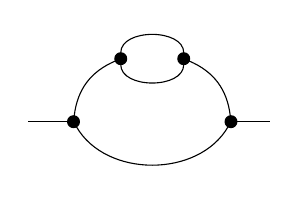
\begin{tikzpicture}
  \begin{feynman}
    % Vertici principali
    \vertex (a);
    \vertex [dot, right=0.5cm of a] (v1) {};
    \vertex [dot, right=2cm of v1] (v4) {};
    \vertex [dot, right=0.5cm of v4] (b);
    
    % Vertici per il loop superiore (posizionati manualmente sopra v1 e v4)
    \vertex [dot, above right=0.8cm and 0.6cm of v1] (v2) {};
    \vertex [dot, above left=0.8cm and 0.6cm of v4] (v3) {};

    \diagram* {
      (a) -- (v1),
      (v4) -- (b),
      % Arco inferiore del cerchio grande
      (v1) -- [bend right=60] (v4),
      % Pezzetti di arco superiore che portano alla bolla
      (v1) -- [bend left=30] (v2),
      (v3) -- [bend left=30] (v4),
      % La bolla superiore (il piccolo cerchio che interrompe)
      (v2) -- [bend left=90] (v3),
      (v2) -- [bend right=90] (v3),
    };
  \end{feynman}
\end{tikzpicture}
\end{equation}
3-gluon vertex with colours
\begin{equation}
    \feynmandiagram[horizontal=a to v, inline=(v.base), layered layout, scale=0.9, transform shape] { 
    a -- [gluon, edge label = \(\textcolor{red}{r}\textcolor{magenta}{\bar{g}}\), pos=0.0] v [dot], v -- [gluon, edge label = \(\textcolor{red}{r}\textcolor{yellow}{\bar{b}}\), pos=0.9] b, v -- [gluon, edge label = \(\textcolor{blue}{b}\textcolor{magenta}{\bar{g}}\), pos=0.9] c 
    };
\end{equation}
quark-quark interaction with colours (version I)
\begin{equation}
    \feynmandiagram[horizontal=v1 to v2, inline=(v1.base), scale=0.9] {
    a [blue, particle=\(q_2\)] -- [fermion] v1, b [red, particle=\(q_2\)] -- [anti fermion] v2, v1 -- [gluon, edge label=\(\textcolor{blue}{b}\textcolor{cyan}{\bar{r}}\), pos=0.5, above=4pt] v2, v1 -- [anti fermion] c [red, particle=\(q_1\)], v2 -- [fermion] d [blue, particle=\(q_1\)]  
    };
\end{equation}
quark-quark interaction with colours (version II)
\begin{equation}
    \feynmandiagram[horizontal=v1 to v2, inline=(v1.base), scale=0.9] {
    a -- [edge label'=\(\textcolor{blue}{q_2}\), fermion, pos=0.2] v1, b -- [anti fermion, edge label=\(\textcolor{red}{q_2}\), pos=0.2] v2, v1 -- [gluon, edge label=\(\textcolor{blue}{b}\textcolor{cyan}{\bar{r}}\), pos=0.5, above=4pt] v2, v1 -- [anti fermion, edge label'=\(\textcolor{red}{q_1}\), pos=0.8] c , v2 -- [fermion, edge label = \(\textcolor{blue}{q_1}\), pos=0.8] d  
    };
\end{equation}
$D_s^+$ decay
\begin{equation}
    \begin{tikzpicture}[scale=0.8, transform shape]
        \begin{feynman}
        % NODI
        \vertex (ds) at (0,0) {\(D_s^+\)};
        \vertex [dot] (v1) at (2,0) {};
        \vertex (taup) at (3,1.4) {\(\tau^+\)};
        \vertex [dot] (v2) at (4,0) {};
        \vertex (x) at (5,1.4) {\(X\)};
        \vertex [dot] (taum) at (5,-1.4) {};
        \vertex (lep) at (7,-0.4) {\(e^-/\mu^-\)};
        \vertex (nubar) at (7,-1.4) {\(\bar{\nu}_e/\bar{\nu}_\mu\)};
        \vertex (nutau) at (6.7,-2.4) {\(\nu_\tau\)};
        
        % PROPAGATORI
        \diagram*{
            (ds) -- (v1),
            (taup) -- (v1),
            (v1) -- [edge label=\(\nu_\tau\)] (v2),
            (v2) -- (x),
            (v2) -- [edge label'=\(\tau^-\)] (taum),
            (taum) -- (lep),
            (taum) -- (nubar),
            (taum) -- (nutau),
        };
        \end{feynman}
    \end{tikzpicture}
\end{equation}
hadrons decay in $e^+ + e^- + X$
\begin{equation}
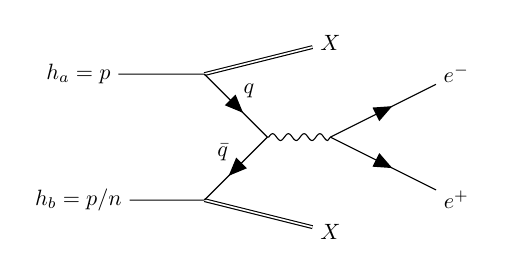
\begin{tikzpicture}[scale=0.8, transform shape]
\begin{feynman}

\vertex (a) at (0,1) {$h_a = p$};
\vertex (b) at (0,-1) {$h_b = p/n$};

\vertex [dot] (v1) at (2,1);
\vertex [dot] (v2) at (2,-1);
\vertex [dot] (q) at (3,0);

\vertex (x1) at (4,1.5) {$X$};
\vertex (x2) at (4,-1.5) {$X$};

\vertex (v3) at (4,0);
\vertex (e1) at (6,1) {$e^-$};
\vertex (e2) at (6,-1) {$e^+$};

\diagram*{
(a) -- (v1),
(b) -- (v2),

(v1) -- [double] (x1),
(v2) -- [double] (x2),

(v1) -- [fermion, edge label=$q$] (q) -- [fermion, edge label'=$\bar q$] (v2),

(q) -- [photon] (v3),

(v3) -- [fermion] (e1),
(v3) -- [fermion] (e2),
};

\end{feynman}
\end{tikzpicture}
\end{equation}
Bare tadpole
\begin{equation}
    \feynmandiagram[inline={([yshift=-0.1cm]current bounding box.center)}, layered layout, horizontal=a to v, scale=0.5, transform shape] { a -- v -- [half left, looseness=1.5] v1 -- [half left, looseness=1.5] v };
\end{equation}
Bare bubble
\begin{equation}
    \feynmandiagram[inline={([yshift=-0.1cm]current bounding box.center)}, layered layout, horizontal=a to b, scale=0.5, transform shape] { a -- v -- [half left, looseness=1.5] v1 -- [half left, looseness=1.5] v, v1 -- b};
\end{equation}
Bare 3-point loop interaction
\begin{equation}
    \feynmandiagram [inline={([yshift=-0.1cm]current bounding box.center)}, scale = 0.5] { a -- [bend left=60] b -- [bend left=60] c -- [bend left=60] a, i1 -- a, i2 -- b,i3 -- c };
\end{equation}
2-loop bubble
\begin{equation}
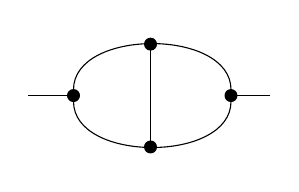
\begin{tikzpicture}[baseline={([yshift=-0.1cm]current bounding box.center)}, scale = 0.6]
  \begin{feynman}
    % Vertici principali
    \vertex (a);
    \vertex [dot, right=0.5cm of a] (v1) {};
    \vertex [dot, right=2cm of v1] (v2) {};
    \vertex [dot, right=0.5cm of v2] (b);
    \vertex [dot, below right=0.6cm and 1.5cm of a] (down) {};
    \vertex [dot, above right=0.6cm and 1.5cm of a] (up) {};

    \diagram* {
      (a) -- (v1),
      (v1) -- [bend right=90] (v2),
      (v2) -- [bend right=90] (v1), (v2) -- (b), (down) -- (up)
    };
  \end{feynman}
\end{tikzpicture}
\end{equation}
Fermion line with a photon
\begin{equation}
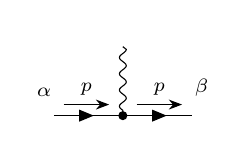
\begin{tikzpicture}
    \begin{feynman}[inline={([yshift=-0.1cm]current bounding box.center)}, scale = 0.8]
    % Vertici principali
    \vertex [label=\ensuremath{\scriptstyle \alpha}] (a) {};
    \vertex [dot, right=1cm of a] (b) {};
    \vertex [above=1cm of b] (c) {};
    \vertex [right=1cm of b, label=\ensuremath{\scriptstyle \beta}] (d) {};

    \diagram* {
      (a) -- [fermion, momentum={[arrow distance=4pt] \ensuremath{\scriptstyle p}}] (b), (b) -- [boson] (c), (b) -- [fermion, momentum={[arrow distance=4pt] \ensuremath{\scriptstyle p}}] (d)
    };
  \end{feynman}
\end{tikzpicture}
\end{equation}
Electromagnetic interaction correction
\begin{equation}
    \feynmandiagram[inline={([yshift=-0.1cm]current bounding box.center)}, horizontal=a to c, scale=0.7, transform shape, rotate=45] { a -- b -- c, b -- [photon] b1 -- [half left, looseness=1.5] v -- [half left, looseness=1.5] b1, v -- [photon] d [dot]};
\end{equation}
Ward-Takahashi identity
\begin{equation}
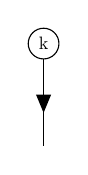
\begin{tikzpicture}[scale=0.65, transform shape, baseline={([yshift=0.2cm]current bounding box.center)}]
    \begin{feynman}
        
        \vertex [draw,circle,minimum size=0.6cm,inner sep=0pt] (k) {k};
        \vertex [below=2cm of k] (down);

        \diagram*{

            (k) -- [fermion] (down),
        };

    \end{feynman}
\end{tikzpicture}
\otimes
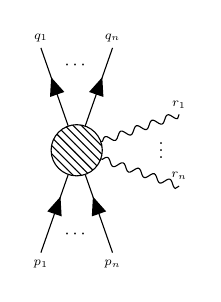
\begin{tikzpicture}[scale=0.65, transform shape, baseline={([yshift=0.2cm]current bounding box.center)}]
    \begin{feynman}
        
        \vertex [blob, minimum size=1cm] (v) {};

        \vertex [above left=2cm and 0.7cm of v, label=\ensuremath{\scriptstyle q_1}] (q1);
        \vertex [above right=2cm and 0.7cm of v, label=\ensuremath{\scriptstyle q_n}] (qn);

        % p
        \vertex [below left=2cm and 0.7cm of v, label={[label distance=0.5pt]below:\ensuremath{\scriptstyle p_1}}] (p1);
        \vertex [below right=2cm and 0.7cm of v, label={[label distance=0.5pt]below:\ensuremath{\scriptstyle p_n}}] (pn);

        % r
        \vertex [above right=0.7 and 2cm of v, label=\ensuremath{\scriptstyle r_1}] (r1);
        \vertex [below right=0.7 and 2cm of v, label=\ensuremath{\scriptstyle r_n}] (rn);

        \diagram*{

            (v) -- [fermion] (q1),
            (v) -- [fermion] (qn),

            (v) -- [anti fermion] (p1),
            (v) -- [anti fermion] (pn),

            (v) -- [photon] (r1),
            (v) -- [photon] (rn)
        };

         \node at ($(q1)!0.5!(qn)+(0,-0.35)$) {$\cdots$};
         \node at ($(p1)!0.5!(pn)+(0,0.35)$) {$\cdots$};
         \node at ($(r1)!0.5!(rn)+(-0.35,0.1)$) {$\vdots$};

    \end{feynman}
\end{tikzpicture}
 = e_R\sum_{i=1}^n
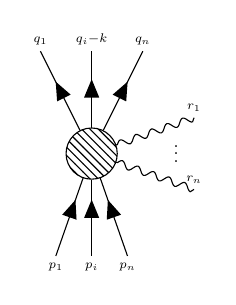
\begin{tikzpicture}[scale=0.65, transform shape, baseline={([yshift=0.2cm]current bounding box.center)}]
    \begin{feynman}
        
        \vertex [blob, minimum size=1cm] (v) {};

        \vertex [above left=2cm and 1cm of v, label=\ensuremath{\scriptstyle q_1}] (q1);
        \vertex [above right=2cm and 1cm of v, label=\ensuremath{\scriptstyle q_n}] (qn);
        \vertex [above =2cm of v, label=\ensuremath{\scriptstyle q_i - k}] (qi-k);

        % p
        \vertex [below left=2cm and 0.7cm of v, label={[label distance=0.5pt]below:\ensuremath{\scriptstyle p_1}}] (p1);
        \vertex [below right=2cm and 0.7cm of v, label={[label distance=0.5pt]below:\ensuremath{\scriptstyle p_n}}] (pn);
        \vertex [below =2cm of v, label={[label distance=0.5pt]below:\ensuremath{\scriptstyle p_i}}] (pi);

        % r
        \vertex [above right=0.7 and 2cm of v, label=\ensuremath{\scriptstyle r_1}] (r1);
        \vertex [below right=0.7 and 2cm of v, label=\ensuremath{\scriptstyle r_n}] (rn);

        \diagram*{

            (v) -- [fermion] (q1),
            (v) -- [fermion] (qn),

            (v) -- [anti fermion] (p1),
            (v) -- [anti fermion] (pn),

            (v) -- [photon] (r1),
            (v) -- [photon] (rn),

            (v) -- [anti fermion] (pi),
            (v) -- [fermion] (qi-k),
        };

         \node at ($(r1)!0.5!(rn)+(-0.35,0.1)$) {$\vdots$};

    \end{feynman}
\end{tikzpicture}
-
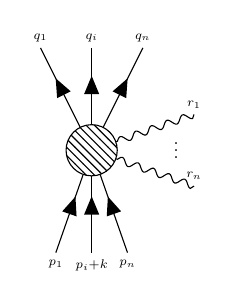
\begin{tikzpicture}[scale=0.65, transform shape, baseline={([yshift=0.2cm]current bounding box.center)}]
    \begin{feynman}
        
        \vertex [blob, minimum size=1cm] (v) {};

        \vertex [above left=2cm and 1cm of v, label=\ensuremath{\scriptstyle q_1}] (q1);
        \vertex [above right=2cm and 1cm of v, label=\ensuremath{\scriptstyle q_n}] (qn);
        \vertex [above =2cm of v, label=\ensuremath{\scriptstyle q_i}] (qi);

        % p
        \vertex [below left=2cm and 0.7cm of v, label={[label distance=0.5pt]below:\ensuremath{\scriptstyle p_1}}] (p1);
        \vertex [below right=2cm and 0.7cm of v, label={[label distance=0.5pt]below:\ensuremath{\scriptstyle p_n}}] (pn);
        \vertex [below =2cm of v, label={[label distance=0.5pt]below:\ensuremath{\scriptstyle p_i+k}}] (pi+k);

        % r
        \vertex [above right=0.7 and 2cm of v, label=\ensuremath{\scriptstyle r_1}] (r1);
        \vertex [below right=0.7 and 2cm of v, label=\ensuremath{\scriptstyle r_n}] (rn);

        \diagram*{

            (v) -- [fermion] (q1),
            (v) -- [fermion] (qn),

            (v) -- [anti fermion] (p1),
            (v) -- [anti fermion] (pn),

            (v) -- [photon] (r1),
            (v) -- [photon] (rn),

            (v) -- [anti fermion] (pi+k),
            (v) -- [fermion] (qi),
        };

         \node at ($(r1)!0.5!(rn)+(-0.35,0.1)$) {$\vdots$};

    \end{feynman}
\end{tikzpicture}
\end{equation}
Fermion with $n$ photons
\begin{equation}
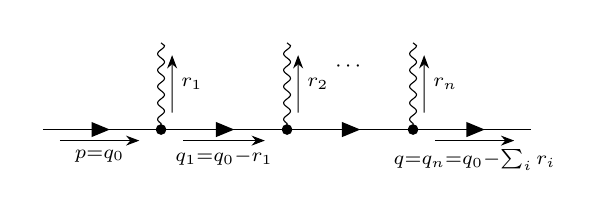
\begin{tikzpicture}[scale=0.8, transform shape, baseline={([yshift=0.2cm]current bounding box.center)}]
    \begin{feynman}
        

        \vertex (a) {};
        \vertex [dot, right=2cm of a] (b) {};
        \vertex [dot, right=2cm of b] (c) {};
        \vertex [dot, right=2cm of c] (d) {};
        \vertex [right=2cm of d] (e) {};

        \vertex[above=1.5 cm of b] (r1) {};
        \vertex[above=1.5 cm of c] (r2) {};
        \vertex [above=1.5 cm of d] (rn) {};
        

        \diagram*{

            (a) -- [fermion, momentum'={[arrow distance=4pt]\ensuremath{\scriptstyle p = q_0}}] (b) -- [fermion, momentum'={[arrow distance=4pt]\ensuremath{\scriptstyle q_1 = q_0 - r_1}}] (c) -- [fermion] (d) -- [fermion, momentum'={[arrow distance=4pt]\ensuremath{\scriptstyle q = q_n = q_0 - \sum_ir_i}}] (e), (b) -- [photon, momentum'={[arrow distance=4pt]\ensuremath{\scriptstyle r_1}}] (r1), (c) -- [photon, momentum'={[arrow distance=4pt]\ensuremath{\scriptstyle r_2}}] (r2), (d) -- [photon, momentum'={[arrow distance=4pt]\ensuremath{\scriptstyle r_n}}] (rn),

        };

         \node at ($(r2)!0.5!(rn)+(0,-0.5)$) {$\cdots$};

    \end{feynman}
\end{tikzpicture}
\end{equation}
Photon insertion
\begin{equation}
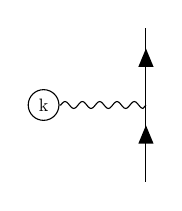
\begin{tikzpicture}[scale=0.65, transform shape, baseline={([yshift=0.2cm]current bounding box.center)}]
    \begin{feynman}
        
        \vertex [draw,circle,minimum size=0.6cm,inner sep=0pt] (k) {k};
        \vertex [right=2cm of k] (right);
        \vertex [above right=1.5cm and 2 cm of k] (up);
        \vertex [below right=1.5cm and 2cm of k] (down);
        

        \diagram*{

            (k) -- [photon] (right), (up) -- [anti fermion] (right) -- [anti fermion] (down)
        };

    \end{feynman}
\end{tikzpicture}
\end{equation}
Fermion line with $n$ photons and a photon insertion
\begin{equation}
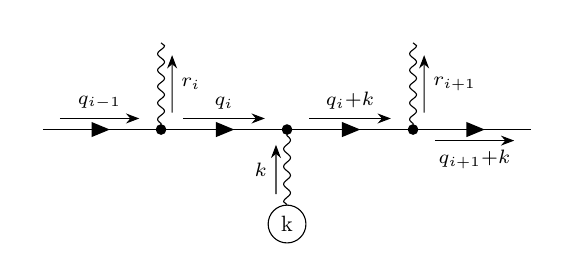
\begin{tikzpicture}[scale=0.8, transform shape, baseline={([yshift=0.2cm]current bounding box.center)}]
    \begin{feynman}
        

        \vertex (a) {};
        \vertex [dot, right=2cm of a] (b) {};
        \vertex [dot, right=2cm of b] (c) {};
        \vertex [dot, right=2cm of c] (d) {};
        \vertex [right=2cm of d] (e) {};

        \vertex [above=1.5 cm of b] (r1) {};
        \vertex [below=1.5 cm of c, draw,circle,minimum size=0.6cm,inner sep=0pt] (r2) {k};
        \vertex [above=1.5 cm of d] (rn) {};
        

        \diagram*{

            (a) -- [fermion, momentum={[arrow distance=4pt]\ensuremath{\scriptstyle q_{i-1}}}] (b) -- [fermion, momentum={[arrow distance=4pt]\ensuremath{\scriptstyle q_i}}] (c) -- [fermion, momentum={[arrow distance=4pt]\ensuremath{\scriptstyle q_i + k}}] (d) -- [fermion, momentum'={[arrow distance=4pt]\ensuremath{\scriptstyle q_{i+1} + k}}] (e),
            (b) -- [photon, momentum'={[arrow distance=4pt]\ensuremath{\scriptstyle r_i}}] (r1), (c) -- [photon, reversed momentum'={[arrow distance=4pt]\ensuremath{\scriptstyle k}}] (r2), (d) -- [photon, momentum'={[arrow distance=4pt]\ensuremath{\scriptstyle r_{i+1}}}] (rn),

        };

    \end{feynman}
\end{tikzpicture}
\end{equation}
3-point vertex correction (in line)
\begin{equation}
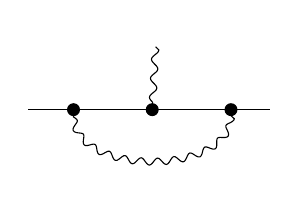
\begin{tikzpicture}
  \begin{feynman}
    % Vertici principali
    \vertex (a);
    \vertex [dot, right=0.5cm of a] (v1) {};
    \vertex [dot, right=2cm of v1] (v2) {};
    \vertex [dot, right=1cm of v1] (centro) {};
    \vertex [dot, right=0.5cm of v2] (b);
    \vertex [above right=0.8cm and 1.5cm of a] (up) {};

    \diagram* {
      (a) -- (v1) -- (v2) -- (b),
      (v1) -- [photon, bend right=90] (v2), (centro) -- [photon] (up),
    };
  \end{feynman}
\end{tikzpicture}
\end{equation}
4-point vertex
\begin{equation}
    \feynmandiagram[inline={([yshift=-0.1cm]current bounding box.center)}, scale = 0.7, horizontal=a to c] { 
    a [label={[yshift=-0.45cm]\ensuremath{\scriptstyle 2}}] -- b [dot] -- d [label=\ensuremath{\scriptstyle 4}], b -- c [label={[yshift=-0.45cm]\ensuremath{\scriptstyle 3}}], b -- e [label=\ensuremath{\scriptstyle 1}]};
\end{equation}
4-point bubble (version I)
\begin{equation}
    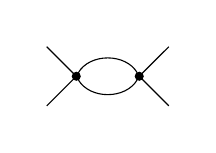
\begin{tikzpicture}
    \begin{feynman}[inline={([yshift=-0.1cm]current bounding box.center)}, scale = 0.7]

    \vertex[dot] (a) {};
    \vertex[dot, right=0.8cm of a] (b) {};
    \vertex[above left=0.5cm and 0.5cm of a] (a1) {};
    \vertex[below left=0.5cm and 0.5cm of a] (a2) {};
    \vertex[above right=0.5cm and 0.5cm of b] (b1) {};
    \vertex[below right=0.5cm and 0.5cm of b] (b2) {};

    \diagram* {
      (a1) -- (a), (a2) -- (a), (a) -- [bend right=60] (b), (b) -- [bend right=60] (a), (b) -- (b1), (b) -- (b2)
    };
  \end{feynman}
\end{tikzpicture}
\end{equation}
4-point bubble (version II)
\begin{equation}
    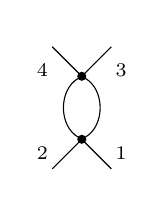
\begin{tikzpicture}
    \begin{feynman}[inline={([yshift=-0.1cm]current bounding box.center)}, scale = 0.7]

    \vertex[dot] (a) {};
    \vertex[dot, below=0.8cm of a] (b) {};
    \vertex[above left=0.5cm and 0.5cm of a, label={[yshift=-0.75cm]\ensuremath{\scriptstyle 4}}] (a1) {};
    \vertex[above right=0.5cm and 0.5cm of a, label={[yshift=-0.75cm]\ensuremath{\scriptstyle 3}}] (a2) {};
    \vertex[below left=0.5cm and 0.5cm of b, label=\ensuremath{\scriptstyle 2}] (b1) {};
    \vertex[below right=0.5cm and 0.5cm of b, label=\ensuremath{\scriptstyle 1}] (b2) {};

    \diagram* {
      (a1) -- (a), (a2) -- (a), (a) -- [bend right=60] (b), (b) -- [bend right=60] (a), (b) -- (b1), (b) -- (b2)
    };
  \end{feynman}
\end{tikzpicture}
\end{equation}
Box contributions
\begin{equation}
    \feynmandiagram[ 
        inline={([yshift=-0.1cm]current bounding box.center)}, 
        scale=0.75, 
        transform shape, 
        horizontal=v1 to v2
    ] { 
        a -- [edge label'=B, pos=0.5] v1, 
        v1 -- v2, 
        v2 -- b, 
        v2 -- v3, 
        v3 -- c, 
        v3 -- v4, 
        v4 -- v1, 
        v4 -- d 
    };
\end{equation}
quark-quark interaction
\begin{equation}
    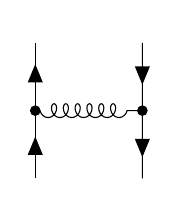
\begin{tikzpicture}[scale=0.8, transform shape, baseline={([yshift=-0.1cm]current bounding box.center)}]
    \begin{feynman}
    
    \vertex [dot] (a) {};
    \vertex [above=1.2cm of a] (v1) {};
    \vertex [below=1.2cm of a] (v2) {};
    \vertex [dot, right=1.7cm of a] (b) {};
    \vertex [above=1.2cm of b] (w1) {};
    \vertex [below=1.2cm of b] (w2) {};

    \diagram* {
      (v2) -- [fermion] (a) -- [fermion] (v1), (w1) -- [fermion] (b) -- [fermion] (w2),
      (a) -- [gluon] (b)
    };
    \end{feynman}
    \end{tikzpicture} 
\end{equation}
Two free quark lines (version I)
\begin{equation}
    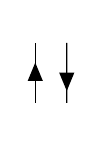
\begin{tikzpicture}[scale=0.8, transform shape, baseline={([yshift=-0.1cm]current bounding box.center)}]
    \begin{feynman}
    
    \vertex (a) {};
    \vertex [above=1.2cm of a] (a1) {};
    
    \vertex [right=0.5cm of a] (b) {};
    \vertex [above=1.2cm of b] (b1) {};

    \diagram* {
      (a) -- [fermion] (a1), (b) -- [anti fermion] (b1)
    };
    \end{feynman}
    \end{tikzpicture} 
\end{equation}
Two free quark lines (version II)
\begin{equation}
    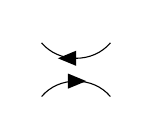
\begin{tikzpicture}[scale=0.8, transform shape, baseline={([yshift=-0.1cm]current bounding box.center)}]
    \begin{feynman}
    
    \vertex (a) {};
    \vertex [right=1.3cm of a] (a1) {};
    
    \vertex [below=1.1cm of a] (b) {};
    \vertex [below=1.1cm of a1] (b1) {};

    \diagram* {
      (a) -- [anti fermion, bend right=50] (a1), (b) -- [fermion, bend left=50] (b1)
    };
    \end{feynman}
    \end{tikzpicture} 
\end{equation}
One free quark line and a quark loop
\begin{equation}
    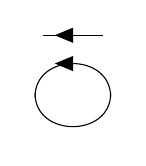
\begin{tikzpicture}[scale=0.8, transform shape, baseline={([yshift=-0.1cm]current bounding box.center)}]
    \begin{feynman}
    
    \vertex (a) {};
    \vertex [right=1.2cm of a] (a1) {};
    \vertex [below=1.1cm of a] (b) {};
    \vertex [below=1.1cm of a1] (b1) {};
    \vertex [above=0.3cm of b] (c) {};
    \vertex [above=0.3cm of b1] (c1) {};

    \diagram* {
      (a) -- [anti fermion] (a1), (b) -- [anti fermion, half left] (b1), (c) -- [half right] (c1)
    };
    \end{feynman}
    \end{tikzpicture} 
\end{equation}
Contribution to $\qbar qgg$ scattering amplitude (version I)
\begin{equation}
    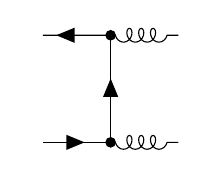
\begin{tikzpicture}[scale=0.8, transform shape, baseline={([yshift=-0.1cm]current bounding box.center)}]
    \begin{feynman}
    
    \vertex [dot] (a) {};
    \vertex [dot, above=1.7cm of a] (b) {};
    
    \vertex [right=1.2cm of a] (v1) {};
    \vertex [left=1.2cm of a] (v2) {};
    \vertex [right=1.2cm of b] (w1) {};
    \vertex [left=1.2cm of b] (w2) {};

    \diagram* {
      (a) -- [fermion] (b), (v2) -- [fermion] (a) -- [gluon] (v1), (w2) -- [anti fermion] (b) -- [gluon] (w1)
    };
    \end{feynman}
    \end{tikzpicture} 
\end{equation}
Contribution to $\qbar qgg$ scattering amplitude (version II)
\begin{equation}
    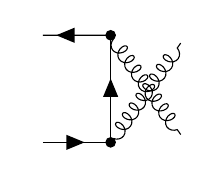
\begin{tikzpicture}[scale=0.8, transform shape, baseline={([yshift=-0.1cm]current bounding box.center)}]
    \begin{feynman}
    
    \vertex [dot] (a) {};
    \vertex [dot, above=1.7cm of a] (b) {};
    
    \vertex [right=1.2cm of a] (v1) {};
    \vertex [left=1.2cm of a] (v2) {};
    \vertex [right=1.2cm of b] (w1) {};
    \vertex [left=1.2cm of b] (w2) {};

    \diagram* {
      (a) -- [fermion] (b), (v2) -- [fermion] (a) -- [gluon] (w1), (w2) -- [anti fermion] (b) -- [gluon] (v1)
    };
    \end{feynman}
    \end{tikzpicture} 
\end{equation}
2-point blob
\begin{equation}
    \feynmandiagram[inline={([yshift=-0.3cm]current bounding box.center)}, horizontal=a to c, scale=0.8, transform shape, layered layout] { 
        a -- [fermion] b [blob] -- [fermion] c, 
        };
\end{equation}
3-point blob
\begin{equation}
    \feynmandiagram[inline={([yshift=-0.3cm]current bounding box.center)}, horizontal=a to c, scale=0.7, transform shape, node distance=1.2cm] { 
        a -- [fermion] b [blob, minimum size=0.3 cm, inner sep=0pt] -- [fermion] c, b -- [fermion] d, 
        };
\end{equation}
4-point blob
\begin{equation}
    \feynmandiagram[inline={([yshift=-0.3cm]current bounding box.center)}, horizontal=a to c, scale=0.8, transform shape, node distance=0.7cm] { 
        a -- [fermion] b [blob, minimum size=0.3 cm, inner sep=0pt] -- [fermion] c, b -- [fermion] d, b -- [fermion] e , 
        };
\end{equation}
Bare triangle interaction
\begin{equation}
    \feynmandiagram[inline={([yshift=-0.1cm]current bounding box.center)}, horizontal=v1 to v2, scale=0.8, transform shape, node distance=0.7cm]{
    a -- [fermion] v1,
    b -- [fermion] v2,
    c -- [fermion] v3,

    v1 -- [fermion] v2
       -- [fermion] v3
       -- [fermion] v1,
    };
\end{equation}
3-point interaction with an internal loop
\begin{equation}
    \feynmandiagram[inline={([yshift=-0.1cm]current bounding box.center)}, horizontal=v to v1, scale=0.8, transform shape] { 
        a -- [fermion] v -- [fermion, half left, looseness=1.5] v1, a1 -- [fermion] v, v1 -- [fermion, half left, looseness=1.5] v, v1 -- [fermion] b , 
        };    
\end{equation}
Fermion line with one loop
\begin{equation}
    \feynmandiagram[inline={([yshift=-0.1cm]current bounding box.center)}, horizontal=a to c, scale=0.8, transform shape, layered layout]{
        a -- [fermion] b [dot]-- [fermion] c,
        b -- [fermion, out=60, in=120, loop, min distance=1.5cm] b,
    };
\end{equation}
3-point loop interaction with arrow
\begin{equation}
    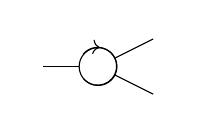
\begin{tikzpicture}[scale=0.8, transform shape, baseline={([yshift=-0.1cm]current bounding box.center)}]
    \begin{feynman}
    
    \vertex (a) {};
    \vertex [right=1cm of a, draw, circle, minimum size=0.6cm, inner sep=0pt] (v) {};
    \vertex [above right=0.5cm and 1cm of v] (b) {};
    \vertex [below right=0.5cm and 1cm of v] (c) {};
    
    \diagram* {
        (a) -- (v),
        (v) -- (b),
        (v) -- (c),
    };
    
    \end{feynman}
    
    % freccia sulla circonferenza
    \draw[
        postaction={
            decorate,
            decoration={
                markings,
                mark=at position 0.2 with {\arrow{>}}
            }
        }
    ] (v.140) arc (140:-140:0.3cm);
    
    \end{tikzpicture}
\end{equation}
Two 3-point loop interactions (version I)
\begin{equation}
    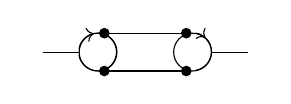
\begin{tikzpicture}[scale=0.8, transform shape, baseline={([yshift=-0.1cm]current bounding box.center)}]
    \begin{feynman}
    
    \vertex (a) {};
    \vertex [right=1cm of a, draw, circle, minimum size=0.6cm, inner sep=0pt] (v) {};
    \vertex [dot, above right=0.3cm and 0.1cm of v] (b) {};
    \vertex [dot, below right=0.3cm and 0.1cm of v] (c) {};
    \vertex [right=1.5cm of v, draw, circle, minimum size=0.6cm, inner sep=0pt] (v1) {};
    \vertex [dot, above left=0.3cm and 0.1cm of v1] (b1) {};
    \vertex [dot, below left=0.3cm and 0.1cm of v1] (c1) {};
    \vertex [right=1cm of v1] (d) {};
    
    
    \diagram* {
        (a) -- (v),
        (b) -- (b1),
        (c) -- (c1),
        (v1) -- (d)
    };
    
    \end{feynman}
    
    % freccia sulla circonferenza
    \draw[
        postaction={
            decorate,
            decoration={
                markings,
                mark=at position 0.2 with {\arrow{>}}
            }
        }
    ] (v.170) arc (170:-170:0.3cm);

    \draw[
        postaction={
            decorate,
            decoration={
                markings,
                mark=at position 0.2 with {\arrow{>}}
            }
        }
    ] (v1.80) arc (80:-80:0.3cm);
    
    \end{tikzpicture}
\end{equation}
Two 3-point loop interactions (version I)
\begin{equation}
    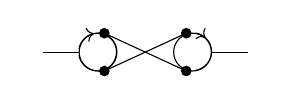
\begin{tikzpicture}[scale=0.8, transform shape, baseline={([yshift=-0.1cm]current bounding box.center)}]
    \begin{feynman}
    
    \vertex (a) {};
    \vertex [right=1cm of a, draw, circle, minimum size=0.6cm, inner sep=0pt] (v) {};
    \vertex [dot, above right=0.3cm and 0.1cm of v] (b) {};
    \vertex [dot, below right=0.3cm and 0.1cm of v] (c) {};
    \vertex [right=1.5cm of v, draw, circle, minimum size=0.6cm, inner sep=0pt] (v1) {};
    \vertex [dot, above left=0.3cm and 0.1cm of v1] (b1) {};
    \vertex [dot, below left=0.3cm and 0.1cm of v1] (c1) {};
    \vertex [right=1cm of v1] (d) {};
    
    
    \diagram* {
        (a) -- (v),
        (b) -- (c1),
        (c) -- (b1),
        (v1) -- (d)
    };
    
    \end{feynman}
    
    % freccia sulla circonferenza
    \draw[
        postaction={
            decorate,
            decoration={
                markings,
                mark=at position 0.2 with {\arrow{>}}
            }
        }
    ] (v.170) arc (170:-170:0.3cm);

    \draw[
        postaction={
            decorate,
            decoration={
                markings,
                mark=at position 0.2 with {\arrow{>}}
            }
        }
    ] (v1.80) arc (80:-80:0.3cm);
    
    \end{tikzpicture}
\end{equation}
Fermion line with two bubbles
\begin{equation}
    \feynmandiagram[inline={([yshift=-0.1cm]current bounding box.center)}, layered layout, horizontal=a to b, scale=0.8, transform shape] { 
        a -- [fermion] v -- [fermion, half left, looseness=1.5] v1, v1 -- [fermion, half left, looseness=1.5] v, v1 -- [fermion] v2, v2 -- [fermion, half left, looseness=1.5] v3, v3 -- [fermion, half left, looseness=1.5] v2, v3 -- [fermion] b
        };    
\end{equation}
2-point loop interaction with arrow and a self-interaction
\begin{equation}
    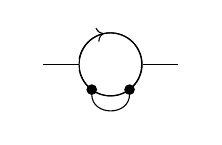
\begin{tikzpicture}[scale=0.8, transform shape, baseline={([yshift=-0.1cm]current bounding box.center)}]
    \begin{feynman}
    
    \vertex (a) {};
    \vertex [right=1.2cm of a, draw, circle, minimum size=1cm, inner sep=0pt] (v) {};
    \vertex [dot, below left=0.4cm and 0.3cm of v] (b) {};
    \vertex [dot, below right=0.4cm and 0.3cm of v] (c) {};
    \vertex [right=1.2cm of v] (d) {};
    
    
    \diagram* {
        (a) -- (v),
        (b) -- [half right] (c), 
        (v) -- (d)
    };
    
    \end{feynman}
    
    % freccia sulla circonferenza
    \draw[
        postaction={
            decorate,
            decoration={
                markings,
                mark=at position 0.2 with {\arrow{>}}
            }
        }
    ] (v.170) arc (170:-170:0.5cm);
    
    \end{tikzpicture}
\end{equation}
Fermion line with a loop interaction 
\begin{equation}
    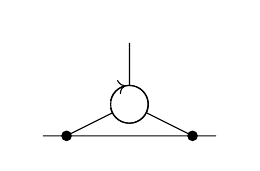
\begin{tikzpicture}[scale=0.8, transform shape, baseline={([yshift=-0.1cm]current bounding box.center)}]
    \begin{feynman}
    
    \vertex [dot] (a) {};
    \vertex [left=0.5cm of a] (i) {};
    \vertex [above right=0.5 and 1cm of a, draw, circle, minimum size=0.6cm, inner sep=0pt] (v) {};
    \vertex [above=1.1cm of v] (b) {};
    \vertex [dot, below right=0.5cm and 1cm of v] (c) {};
    \vertex [right=0.5cm of c] (f) {};
    
    \diagram* {
        (a) -- (v),
        (v) -- (b),
        (v) -- (c),
        (i) -- (f)
    };
    
    \end{feynman}
    
    % freccia sulla circonferenza
    \draw[
        postaction={
            decorate,
            decoration={
                markings,
                mark=at position 0.2 with {\arrow{>}}
            }
        }
    ] (v.170) arc (170:-170:0.3cm);
    
    \end{tikzpicture}
\end{equation}
General scattering process (blob)
\begin{equation}
    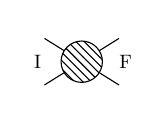
\begin{tikzpicture}[scale=0.7, transform shape, baseline={([yshift=-0.1cm]current bounding box.center)}]
    \begin{feynman}
    
    \vertex (i) {I};
    \vertex[right=0.8cm of i, blob] (v) {};
    \vertex[above=0.5cm of i] (a) {};
    \vertex[below=0.5cm of i] (b) {};
    \vertex[right=0.8cm of v] (f) {F};
    \vertex[above=0.5cm of f] (e) {};
    \vertex[below=0.5cm of f] (g) {};
    
    \diagram* {
        (a) -- (v), (b) -- (v), (v) -- (e), (v) -- (g)
    };
    
    \end{feynman}
    \end{tikzpicture}
\end{equation}
General scattering process (circle)
\begin{equation}
    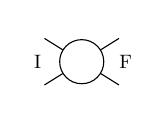
\begin{tikzpicture}[scale=0.7, transform shape, baseline={([yshift=-0.1cm]current bounding box.center)}]
    \begin{feynman}
    
    \vertex (i) {I};
    \vertex[right=0.8cm of i, draw, circle, minimum size=0.8cm, inner sep=0pt] (v) {};
    \vertex[above=0.5cm of i] (a) {};
    \vertex[below=0.5cm of i] (b) {};
    \vertex[right=0.8cm of v] (f) {F};
    \vertex[above=0.5cm of f] (e) {};
    \vertex[below=0.5cm of f] (g) {};
    
    \diagram* {
        (a) -- (v), (b) -- (v), (v) -- (e), (v) -- (g)
    };
    
    \end{feynman}
    \end{tikzpicture}
\end{equation}
General scattering process with three final states
\begin{equation}
    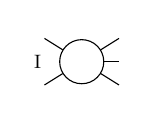
\begin{tikzpicture}[scale=0.7, transform shape, baseline={([yshift=-0.1cm]current bounding box.center)}]
    \begin{feynman}
    
    \vertex (i) {I};
    \vertex[right=0.8cm of i, draw, circle, minimum size=0.8cm, inner sep=0pt] (v) {};
    \vertex[above=0.5cm of i] (a) {};
    \vertex[below=0.5cm of i] (b) {};
    \vertex[right=0.8cm of v] (f) {};
    \vertex[above=0.5cm of f] (e) {};
    \vertex[below=0.5cm of f] (g) {};
    
    \diagram* {
        (a) -- (v), (b) -- (v), (v) -- (e), (v) -- (g), (v) -- (f)
    };
    
    \end{feynman}
    \end{tikzpicture}
\end{equation}
3-point loop interaction with momenta
\begin{equation}
    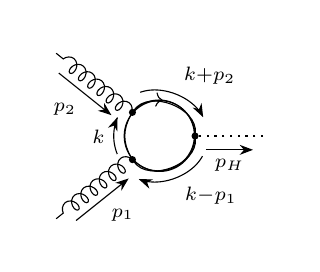
\begin{tikzpicture}[scale=1.5, transform shape, baseline={([yshift=-0.1cm]current bounding box.center)}]
    \begin{feynman}
    
    \vertex (a) {};
    \vertex [left=1cm of a, draw, circle, minimum size=0.6cm, inner sep=0pt] (v) {};
    \vertex [above left=0.8cm and 1cm of v] (b) {};
    \vertex [below left=0.8cm and 1cm of v] (c) {};

    \vertex [dot, minimum size=0.05cm, above left=0.2cm and 0.23cm of v] (q) {};
    \vertex [dot, minimum size=0.05cm, below left=0.2cm and 0.23cm of v] (q1) {};
    \vertex [dot, minimum size=0.05cm, left=0.7cm of a] (q2) {};
    
    \diagram* {
        (a) -- [ghost, reversed momentum={[arrow distance=5pt]\ensuremath{\scriptstyle p_H}}] (v),
        (v) -- [gluon, reversed momentum={[arrow distance=5pt]\ensuremath{\scriptstyle p_2}}] (b),
        (v) -- [gluon, reversed momentum={[arrow distance=5pt]\ensuremath{\scriptstyle p_1}}] (c),

        (q1) -- [bend left=30, momentum={[arrow distance=4pt]\ensuremath{\scriptstyle k}}] (q), (q) -- [bend left=75, momentum={[arrow distance=4pt]\ensuremath{\scriptstyle k + p_2}}] (q2), (q2) -- [bend left=75, momentum={[arrow distance=4pt]\ensuremath{\scriptstyle k - p_1}}] (q1)
    };
    
    \end{feynman}
    
    % freccia sulla circonferenza
    \draw[
        postaction={
            decorate,
            decoration={
                markings,
                mark=at position 0.2 with {\arrow{>}}
            }
        }
    ] (v.140) arc (140:-140:0.3cm);
    
    \end{tikzpicture}
\end{equation}
2-loop bubble with arrow
\begin{equation}
    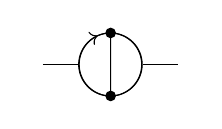
\begin{tikzpicture}[scale=0.8, transform shape, baseline={([yshift=-0.1cm]current bounding box.center)}]
    \begin{feynman}
    
    \vertex (a) {};
    \vertex [right=1.2cm of a, draw, circle, minimum size=1cm, inner sep=0pt] (v) {};
    \vertex [dot, below=0.5cm of v] (b) {};
    \vertex [dot, above=0.5cm of v] (c) {};
    \vertex [right=1.2cm of v] (d) {};
    
    
    \diagram* {
        (a) -- (v),
        (b) -- (c), 
        (v) -- (d)
    };
    
    \end{feynman}
    
    % freccia sulla circonferenza
    \draw[
        postaction={
            decorate,
            decoration={
                markings,
                mark=at position 0.2 with {\arrow{>}}
            }
        }
    ] (v.190) arc (190:-190:0.5cm);
    
    \end{tikzpicture}
\end{equation}
Fermion line with two bubble with arrows
\begin{equation}
    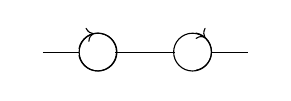
\begin{tikzpicture}[scale=0.8, transform shape, baseline={([yshift=-0.1cm]current bounding box.center)}]
    \begin{feynman}
    
    \vertex (a) {};
    \vertex [right=1cm of a, draw, circle, minimum size=0.6cm, inner sep=0pt] (v) {};
    \vertex [right=0.15cm of v] (b) {};
    \vertex [right=1.5cm of v, draw, circle, minimum size=0.6cm, inner sep=0pt] (v1) {};
    \vertex [left=0.15cm of v1] (b1) {};
    \vertex [right=1cm of v1] (d) {};
    
    
    \diagram* {
        (a) -- (v),
        (b) -- (b1),
        (v1) -- (d)
    };
    
    \end{feynman}
    
    % freccia sulla circonferenza
    \draw[
        postaction={
            decorate,
            decoration={
                markings,
                mark=at position 0.2 with {\arrow{>}}
            }
        }
    ] (v.170) arc (170:-170:0.3cm);

    \draw[
        postaction={
            decorate,
            decoration={
                markings,
                mark=at position 0.2 with {\arrow{>}}
            }
        }
    ] (v1.80) arc (80:-80:0.3cm);
    
    \end{tikzpicture}
\end{equation}
Two tadpoles with arrows
\begin{equation}
    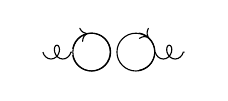
\begin{tikzpicture}[scale=0.8, transform shape, baseline={([yshift=-0.1cm]current bounding box.center)}]
    \begin{feynman}
    
    \vertex (a) {};
    \vertex [right=0.9cm of a, draw, circle, minimum size=0.6cm, inner sep=0pt] (v) {};
    \vertex [right=0.15cm of v] (b) {};
    \vertex [right=0.7cm of v, draw, circle, minimum size=0.6cm, inner sep=0pt] (v1) {};
    \vertex [left=0.15cm of v1] (b1) {};
    \vertex [right=0.9cm of v1] (d) {};
    
    
    \diagram* {
        (a) --[gluon] (v),
        (b) -- [opacity=0] (b1),
        (v1) -- [gluon] (d)
    };
    
    \end{feynman}
    
    % freccia sulla circonferenza
    \draw[
        postaction={
            decorate,
            decoration={
                markings,
                mark=at position 0.2 with {\arrow{>}}
            }
        }
    ] (v.170) arc (170:-170:0.3cm);

    \draw[
        postaction={
            decorate,
            decoration={
                markings,
                mark=at position 0.2 with {\arrow{>}}
            }
        }
    ] (v1.80) arc (80:-80:0.3cm);
    
    \end{tikzpicture}
\end{equation}

\end{document}
